\documentclass[tikz]{standalone}
\usepackage{tikz}
\usetikzlibrary{
	shapes,
	snakes,
	calc,
	decorations,
	decorations.markings,
	decorations.text,
	decorations.pathreplacing}
	
\begin{document}
%	\begin{tikzpicture}[scale=1,auto,every text node part/.style={align=center}]
%	
%		% Parse Tree
%%%        \node (lab1) at (0,4) {\bf Parse Tree};
%        \node (S) at (0,3) {$S$(after twenty five comes twenty six)\\\tiny$S(XY)$};
%        \node (S-A1) at (0,1.5) {\tiny$A_1(X,Y)$\\$A_1$(after twenty five, comes twenty six)\\\tiny$A_1(XY,UV)$};
%        \node (A1-A2) at (-2,0) {\tiny$A_2(X,U)$\\$A_2$(after, comes).\\};
%        \node (A1-A3) at ( 2,0) {\tiny$A_3(Y,V)$\\$A_3$(twenty five, twenty six)\\\tiny$A_3(XY,UV)$};
%        \node (A3-A4) at ( 0,-1.5) {\tiny$A_4(X,U)$\\$A_4$(twenty, twenty).};
%        \node (A3-A5) at ( 4,-1.5) {\tiny$A_5(Y,V)$\\$A_5$(five, six).};
%
%    	\draw [<-] (S)     to (S-A1);
%		\draw [<-] (S-A1)  to (A1-A2);
%		\draw [<-] (S-A1)  to (A1-A3);
%		\draw [<-] (A1-A3) to (A3-A4);
%		\draw [<-] (A1-A3) to (A3-A5);
%        
%        % Rule listings
%%%       \node[anchor=west] (lab2) at (5,5) {\bf Applied Rules};
%        \node[anchor=west] (R1) at (1,2.25) {\tiny using $S(XY) \leftarrow A_1(X,Y).$};
%        \node[anchor=west] (R2.west) at (2.5,0.75) {\tiny using $A_1(XY,UV) \leftarrow A_2(X,U),\,A_3(Y,V).$};
%        \node[anchor=west] (R3.west) at (4,-0.75) {\tiny using $A_3(XY,UV) \leftarrow A_4(X,U),\,A_5(Y,V).$};
%	\end{tikzpicture}
	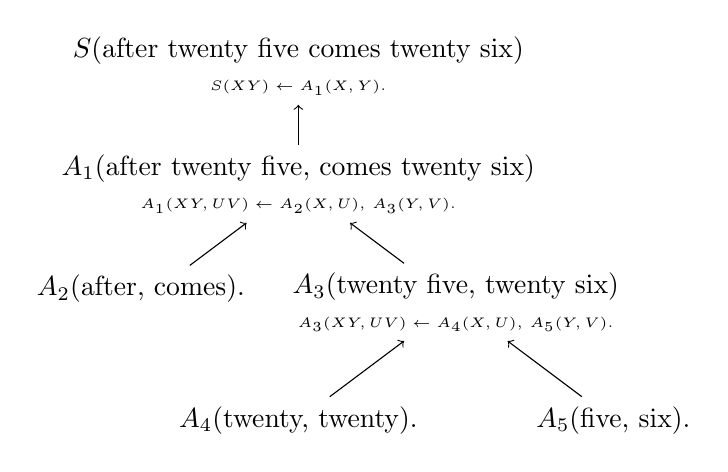
\begin{tikzpicture}[scale=1,auto,every text node part/.style={align=center}]
	
		% Parse Tree
        \node (S) at (0,3) {$S$(after twenty five comes twenty six)\\\tiny$S(XY) \leftarrow A_1(X,Y).$};
        \node (S-A1) at (0,1.5) {$A_1$(after twenty five, comes twenty six)\\\tiny$A_1(XY,UV) \leftarrow A_2(X,U),\,A_3(Y,V).$};
        \node (A1-A2) at (-2,0) {$A_2$(after, comes).\\};
        \node (A1-A3) at ( 2,0) {$A_3$(twenty five, twenty six)\\\tiny$A_3(XY,UV) \leftarrow A_4(X,U),\,A_5(Y,V).$};
        \node (A3-A4) at ( 0,-1.5) {$A_4$(twenty, twenty).};
        \node (A3-A5) at ( 4,-1.5) {$A_5$(five, six).};

    	\draw [<-] (S)     to (S-A1);
		\draw [<-] (S-A1)  to (A1-A2);
		\draw [<-] (S-A1)  to (A1-A3);
		\draw [<-] (A1-A3) to (A3-A4);
		\draw [<-] (A1-A3) to (A3-A5);

	\end{tikzpicture}
\end{document}